\chapter{Relativistische dynamica}\label{ch:b3:relativistic-dynamics}

In 1964 filmde William Bertozzi elektronen die door een lineaire
versneller raasden: elke puls kreeg een gemeten energie mee, en zijn
snelheid werd over \qty{8.4}{m} vluchtweg geklokt. Newton voorspelde dat
elektronen van \qty{15}{MeV} met acht keer de lichtsnelheid zouden
vliegen; de stopwatch zei $0.9999c$ en weigerde verder te gaan, hoe hard
de elektronen ook werden geduwd. De kinematica vertelde ons in het vorige
hoofdstuk dat $c$ een grens is; de dynamica moet nu verklaren wat er met
het duwen gebeurt --- waar de arbeid heen gaat wanneer de snelheid niet
meer groeit. Het antwoord herordent de mechanica rond een nieuwe impuls
en een nieuwe energie, verenigd in de beroemdste vergelijking van de
natuurkunde: opgeslagen energie is massa, en massa is energie die ergens
woont, $E = mc^2$. Dit hoofdstuk bouwt die dynamica op en zet haar dan
aan het werk waar zij dagelijks leeft --- radioactief verval,
deeltjesbotsingen en de versnellers die beweging in nieuwe materie
omzetten.

\section{Impuls en energie, opnieuw opgebouwd}

\begin{remark}[Waarom $m\vect v$ moest wijken]\label{rem:b3:relativistic-dynamics:why}
De klassieke impuls $m\vect v$ blijft in elk stelsel behouden \emph{als}
snelheden zich à la Galilei transformeren. Dat doen zij niet
(\cref{prop:b3:relativistic-kinematics:addition}): een botsing die in het
ene stelsel $\sum m\vect v$ behoudt, doet dat in een ander niet, zodat de
oude impuls geen natuurwet kan zijn --- hooguit een schaduw van een wet
bij lage snelheid. De herstelling is de snelheid met de \emph{eigen} klok
van het deeltje te meten: $\dd\vect r/\dd\tau =
\gamma\,\vect v$
transformeert netjes, en $m\,\dd\vect r/\dd\tau$ blijkt in alle stelsels
tegelijk behouden te blijven.
\end{remark}

\begin{definition}[Relativistische impuls en energie]\label{def:b3:relativistic-dynamics:momentum-energy}
\index{relativistische impuls}\index{relativistische energie}\index{rustenergie}
Een deeltje met massa $m$ en snelheid $\vect v$ ($\gamma = 1/\sqrt{1 -
v^2/c^2}$) draagt de impuls en de energie
\[
\vect p = \gamma m\vect v , \qquad
E = \gamma mc^2 .
\]
In rust is $E_0 = mc^2$: de \emph{rustenergie}. De kinetische energie is
wat de beweging toevoegt, $E_k = E - mc^2 = (\gamma - 1)mc^2$, wat voor
$v
\ll c$ herleidt tot de vertrouwde $\tfrac12 mv^2$ (ontwikkel
$\gamma$). In elk geïsoleerd proces blijven de totale $\vect p$ en de
totale $E$ --- rustenergieën inbegrepen --- behouden.
\end{definition}

\begin{theorem}[De energie--impulsbetrekking]\label{thm:b3:relativistic-dynamics:relation}
\index{energie--impulsbetrekking}
Voor elk deeltje geldt
\[
E^2 = (pc)^2 + (mc^2)^2 ,
\qquad
\vect v = \frac{\vect p\,c^2}{E} :
\]
de combinatie $E^2 - p^2c^2 = m^2c^4$ heeft in elk stelsel dezelfde
waarde --- zij is voor energie en impuls wat het interval voor tijd en
ruimte is. Twee regimes: bij lage snelheid $E \approx mc^2 + p^2/2m$; bij
hoge energie ($E \gg mc^2$) is $E \approx pc$ en $v \to c$: harder duwen
voegt energie en impuls toe, en vrijwel geen snelheid.
\end{theorem}

\begin{proof}
$E^2 - p^2c^2 = \gamma^2m^2c^4(1 - v^2/c^2) = m^2c^4$; en $pc^2/E =
\gamma mvc^2/\gamma mc^2 = v$. De stelselinvariantie volgt omdat $m$ en
$c$ niet van het stelsel afhangen.
\end{proof}

\begin{proposition}[Massaloze deeltjes]\label{prop:b3:relativistic-dynamics:massless}
\index{foton!impuls}
Een deeltje met massa nul heeft $E = pc$ en beweegt in elk stelsel exact
met $c$; het kan niet worden afgeremd, alleen roodverschoven. Het foton
is het standaardgeval: $E = h\nu$ en $p = h\nu/c = h/\lambda$ --- de
betrekkingen van Planck en Einstein uit het volume van jaar 1, nu gezien
als de hoek $m = 0$ van de mechanica.
\end{proposition}

\begin{proof}
Stel $m = 0$ in \cref{thm:b3:relativistic-dynamics:relation}: $E = pc$ en
$v = pc^2/E = c$.
\end{proof}

\begin{omfigure}
\begin{tikzpicture}
  \begin{axis}[omaxis, axis x line=bottom, axis y line=left,
    width=6.6cm, height=5.4cm, xmin=0, xmax=4.3, ymin=0, ymax=1.35,
    xlabel={$E_k/mc^2$}, ylabel={$v^2/c^2$},
    xlabel style={at={(axis description cs:0.5,-0.1)}, anchor=north},
    xtick={1,2,3,4}, ytick={0.5,1}, clip=false]
    \addplot[omExo, dashed, thick, domain=0:0.68] {2*x};
    \addplot[omDef, very thick, domain=0:4.3, samples=80] {1 - 1/(1+x)^2};
    \addplot[gray, dashed, domain=0:4.3] {1};
    \node[omExo, font=\scriptsize, anchor=west] at (axis cs:0.8,1.24) {Newton: $v^2 = 2E_k/m$};
    \node[omDef, font=\scriptsize, anchor=west] at (axis cs:2.0,0.82) {relativiteit};
    \fill[omThm] (axis cs:0.87,0.714) circle (1.6pt);
    \fill[omThm] (axis cs:1.96,0.886) circle (1.6pt);
    \fill[omThm] (axis cs:2.94,0.935) circle (1.6pt);
  \end{axis}
  \begin{axis}[omaxis, axis x line=bottom, axis y line=left,
    width=6.6cm, height=5.4cm, xmin=0, xmax=3, ymin=0, ymax=3.3,
    xshift=7.2cm,
    xlabel={$pc/mc^2$}, ylabel={$E/mc^2$},
    xlabel style={at={(axis description cs:0.5,-0.1)}, anchor=north},
    xtick={1,2,3}, ytick={1,2,3}, clip=false]
    \addplot[omDef, very thick, domain=0:3, samples=60] {sqrt(1+x*x)};
    \addplot[omExo, dashed, domain=0:3] {x};
    \draw[<->, omThm] (axis cs:0,0.04) -- (axis cs:0,0.96);
    \node[omThm, font=\scriptsize, anchor=west] at (axis cs:0.06,0.5) {$mc^2$};
    \node[omExo, font=\scriptsize, anchor=north west] at (axis cs:2.1,2.0) {$E = pc$ (licht)};
    \node[omDef, font=\scriptsize, anchor=south east] at (axis cs:2.9,3.1) {$E = \sqrt{p^2c^2 + m^2c^4}$};
  \end{axis}
\end{tikzpicture}

{\small Links: het experiment van Bertozzi over de ``uiterste snelheid''
--- de gemeten elektronsnelheden (stippen) volgen de relativistische
kromme en verzadigen bij $c$, terwijl de rechte van Newton er straal
voorbij zeilt. Rechts: de energie--impulshyperbool; haar afstand tot nul
bij $p = 0$ is de \omterm{def:b3:relativistic-dynamics:momentum-energy}{rustenergie}, haar asymptoot de $E = pc$ van het foton.}
\end{omfigure}

\begin{example}[Ordes van grootte]\label{ex:b3:relativistic-dynamics:orders}
De deeltjesfysica telt energie in elektronvolt en massa's in
$\unit{MeV}/c^2$: elektron $0.511$, proton $938.3$, muon $105.7$, pion
$139.6$. Een elektron met kinetische energie \qty{1}{MeV} heeft $\gamma =
2.96$ en $v = 0.94c$ --- al volledig relativistisch, en daarom blijft de
elektronica klassiek (\unit{eV}) en de kernfysica niet (\unit{MeV}). Een
LHC-proton van \qty{6.8}{TeV} heeft $\gamma = 7250$ en blijft slechts
\qty{2.9}{m/s} achter op een foton.
\end{example}

\section{Massa is energie die ergens woont}

\begin{theorem}[Gelijkwaardigheid van massa en energie]\label{thm:b3:relativistic-dynamics:emc2}
\index{gelijkwaardigheid van massa en energie}\index{massadefect}
De massa van een lichaam is de totale energie van zijn inhoud, gedeeld
door $c^2$, gemeten in zijn ruststelsel: verwarm een lichaam, span zijn
veer op, breng zijn atomen in aangeslagen toestand, en het weegt
$\Delta E/c^2$ meer; bind zijn delen samen, en het weegt \emph{minder}
met de bindingsenergie gedeeld door $c^2$ --- het \emph{\omterm{thm:b3:relativistic-dynamics:emc2}{massadefect}}.
Omgekeerd kan \omterm{def:b3:relativistic-dynamics:momentum-energy}{rustenergie} vrijkomen: telkens wanneer de eindmassa's samen
minder zijn dan de beginmassa's, komt het verschil $\Delta m\,c^2$ als
kinetische energie of straling tevoorschijn.
\end{theorem}
\admitted

\begin{example}[De boekhouding van $c^2$]\label{ex:b3:relativistic-dynamics:ledger}
$c^2 = \qty{9e16}{J/kg}$: één gram massaverschil is \qty{9e13}{J}, de
energie van een kleine stad voor een dag. Chemische bindingen (enkele eV
per molecuul) verschuiven massa's met delen op $10^{10}$ --- voor altijd
onweegbaar, en daarom heeft de scheikunde het nooit gemerkt. De
kernbinding verschuift ze met bijna $1\%$: helium weegt $0.7\%$ minder
dan zijn vier waterstofbestanddelen, en die ontbrekende fractie, die als
licht van de zon stroomt, kost haar elke seconde $\Delta m = L_\odot/c^2 =
\qty{4.3e9}{kg}$ --- vier miljoen ton zonneschijn. Annihilatie
vereffent de hele rekening: een elektron dat een positron ontmoet laat
niets achter dan twee fotonen van elk \qty{511}{keV}, het signaal waarmee
PET-scanners een levend brein bekijken.
\end{example}

\begin{remark}[Wat ``omzetting'' betekent]\label{rem:b3:relativistic-dynamics:conversion}
Er ``verandert'' niets stoffelijks in energie: de totale energie bleef
aldoor behouden. Wat verandert is haar \emph{woonplaats} --- van
\omterm{def:b3:relativistic-dynamics:momentum-energy}{rustenergie}, die weegt, naar kinetische energie en straling, die vliegen.
De diepe uitspraak van $E = mc^2$ is dat traagheid zelf een
energie-inhoud is: een doos heet gas verzet zich meer tegen versnelling
dan dezelfde doos koud.
\end{remark}

\section{Botsingen en vervallen}

\begin{definition}[Viererimpuls en invariante massa]\label{def:b3:relativistic-dynamics:four-momentum}
\index{viererimpuls}\index{invariante massa}
Bundel de energie en de impuls van een deeltje tot zijn
\emph{viererimpuls} $P = (E/c, \vect p)$. Voor een stelsel deeltjes
telt men componentsgewijs op: $E_{\text{tot}} = \sum E_i$, $\vect p_{\text{tot}} = \sum\vect p_i$. De \emph{invariante massa} $M$ van het
stelsel wordt gedefinieerd door
\[
M^2c^4 = E_{\text{tot}}^2 - \|\vect p_{\text{tot}}\|^2c^2 :
\]
in elk stelsel hetzelfde getal, gelijk aan de totale energie (gedeeld
door $c^2$) in het \emph{impulsmiddelpuntstelsel}, waar $\vect p_{\text{tot}} = \vect 0$. Merk op dat $M$ de som van de massa's van de
delen overtreft zodra die ten opzichte van elkaar bewegen --- twee
fotonen die uiteenvliegen hebben $M > 0$, hoewel elk ervan massaloos is.
\end{definition}

\begin{method}[Een relativistische botsing oplossen]\label{met:b3:relativistic-dynamics:method}
(1) Schrijf het behoud van \omterm{def:b3:relativistic-dynamics:four-momentum}{viererimpuls} op: $E$ en $\vect p$ samen, nooit
één van beide alleen. (2) Bereken de invariant $E^2 - p^2c^2$ van welke
bundel dan ook die handig is --- zij mag in het eenvoudigste stelsel
worden uitgerekend en in elk ander gebruikt. (3) Drempels: een reactie is
mogelijk zodra de \omterm{def:b3:relativistic-dynamics:four-momentum}{invariante massa} van de begintoestand de opgetelde
rustmassa's van de eindtoestand haalt. (4) Verval in rust: de impulsen
van de producten zijn tegengesteld en even groot; hun energieën volgen
uit de massa's alleen. (5) Reken pas op het allerlaatst, als ernaar
gevraagd wordt, om naar snelheden via $v = pc^2/E$.
\end{method}

\begin{example}[De vingerafdruk van het pion]\label{ex:b3:relativistic-dynamics:pion}
Een geladen pion in rust vervalt volgens $\pi^+ \to \mu^+ + \nu$ (het
neutrino is in de praktijk massaloos). Behoud van impuls stuurt de
producten rug aan rug weg met dezelfde $p$; het energiebehoud luidt
$m_\pi c^2 =
\sqrt{p^2c^2 + m_\mu^2c^4} + pc$. Oplossen geeft
\[
pc = \frac{(m_\pi^2 - m_\mu^2)c^2}{2m_\pi} = \qty{29.8}{MeV} ,
\]
zodat elk muon uit een pion dat in rust vervalt met precies
\qty{4.1}{MeV} kinetische energie geboren wordt --- een mono-energetische
lijn, en de waarneming ervan (Powell, 1947) is hoe de massa van het pion
voor het eerst werd gewogen. Tweelichaamsvervallen geven altijd zulke
lijnen; drielichaamsvervallen smeren ze uit tot spectra, en precies zo
werd het neutrino in het kernverval $\beta$ voor het eerst vermoed.
\end{example}

\begin{proposition}[Drempels: de tirannie van het vaste trefplaatje]\label{prop:b3:relativistic-dynamics:threshold}
\index{drempelenergie}\index{botser}
Om nieuwe deeltjes te maken is alleen de energie $Mc^2$ in het
\emph{impulsmiddelpuntstelsel} beschikbaar. Een bundel met energie $E$
die een trefplaatje met massa $m_{\text{t}}$ in rust treft, levert
\[
M^2c^4 = m_{\text{b}}^2c^4 + m_{\text{t}}^2c^4 +
2\,E\,m_{\text{t}}c^2 :
\]
de bruikbare energie groeit slechts als $\sqrt E$ --- de rest gaat
verloren aan het vooruitduwen van het puin. Twee identieke bundels die
frontaal botsen leveren $Mc^2 = 2E$: alles bruikbaar. Deze ene formule is
de reden dat de machines aan de grens botsers zijn
(\cref{pb:b3:relativistic-dynamics:1}).
\end{proposition}

\begin{proof}
Bereken $E_{\text{tot}}^2 - p_{\text{tot}}^2c^2$ in het lab:
$(E + m_{\text{t}}c^2)^2 - p^2c^2$ met $p$ de bundelimpuls; werk uit en
gebruik $E^2 - p^2c^2 = m_{\text{b}}^2c^4$. Voor de botser is $\vect p_{\text{tot}} = \vect 0$ en $Mc^2 = E_{\text{tot}}$.
\end{proof}

\begin{omfigure}
\begin{tikzpicture}[font=\small, >=Stealth]
  % fixed target
  \begin{scope}
    \fill[omDef] (0,0) circle (2.6pt);
    \draw[->, omDef, very thick] (0.15,0) -- (1.45,0);
    \node[font=\footnotesize] at (0.0,0.42) {$E$};
    \fill[omExo] (2.3,0) circle (2.6pt);
    \node[font=\footnotesize] at (2.3,0.42) {in rust};
    \draw[->, thick] (3.1,0) -- (3.8,0);
    \fill[gray] (4.6,0) circle (2.6pt);
    \draw[->, gray, very thick] (4.75,0) -- (5.9,0);
    \draw[->, gray, thick] (4.68,0.12) -- (5.5,0.62);
    \draw[->, gray, thick] (4.68,-0.12) -- (5.5,-0.62);
    \node[align=center, font=\footnotesize] at (2.9,-1.25)
      {vast trefplaatje: $Mc^2 \approx \sqrt{2\,E\,m_{\text{t}}c^2}$\\het puin houdt de meeste energie};
  \end{scope}
  % collider
  \begin{scope}[xshift=8.3cm]
    \fill[omDef] (0,0) circle (2.6pt);
    \draw[->, omDef, very thick] (0.15,0) -- (1.45,0);
    \node[font=\footnotesize] at (0.0,0.42) {$E$};
    \fill[omThm] (3.4,0) circle (2.6pt);
    \draw[->, omThm, very thick] (3.25,0) -- (1.95,0);
    \node[font=\footnotesize] at (3.4,0.42) {$E$};
    \node[align=center, font=\footnotesize] at (1.7,-1.25)
      {botser: $Mc^2 = 2E$\\elke joule is beschikbaar};
  \end{scope}
\end{tikzpicture}

{\small Materie uit beweging maken: op een vast trefplaatje dwingt het
impulsbehoud de producten door te vliegen, en de bruikbare energie in het
impulsmiddelpuntstelsel groeit slechts als $\sqrt E$; bij een frontale
botsing is zij de volle $2E$.}
\end{omfigure}

\section{Kracht en de machines}

\begin{proposition}[Relativistische bewegingsvergelijking]\label{prop:b3:relativistic-dynamics:force}
\index{synchrotron}
De wet van Newton overleeft in de vorm
\[
\vect F = \frac{\dd\vect p}{\dd t} = \frac{\dd(\gamma m\vect v)}
{\dd t} , \qquad
\frac{\dd E}{\dd t} = \vect F\cdot\vect v .
\]
Een magneetveld, dat altijd loodrecht op $\vect v$ staat, verandert de
energie niet en buigt de baan tot een cirkel met straal
\[
r = \frac{p}{qB}
\]
--- dezelfde formule als in het volume van jaar 1, met de relativistische
$p$. Maar de omloopfrequentie $qB/\gamma m$ \emph{daalt} nu naarmate het
deeltje energie wint: het duwtje met vaste frequentie van het cyclotron
raakt rond de schaal van de MeV uit de pas, en de machines voor hoge
energie --- de \emph{synchrotrons} --- laten in plaats daarvan hun veld
en hun frequentie meelopen met $\gamma$, zodat de bundel op één ring
blijft.
\end{proposition}

\begin{proof}[Gedeeltelijk bewijs]
De krachtwet is de definitie van een dynamica die bij de nieuwe impuls
past ($\dd E/\dd t$ volgt uit $E^2 = p^2c^2 + m^2c^4$: $E\,\dot E = c^2\vect p\cdot\dot{\vect p}$). Voor de cirkel: $|\dd\vect p/\dd t| = qvB$ met constante $|\vect p|$ betekent dat de impulsvector met snelheid
$qvB/p$ ronddraait, zodat de straal $v/(qvB/p) = p/qB$ is.
\end{proof}

\begin{example}[De LHC lezen als een opgave]\label{ex:b3:relativistic-dynamics:lhc}
Protonen met $E = \qty{6.8}{TeV}$ in dipolen met $B = \qty{8.3}{T}$: $p \approx E/c$ (ultrarelativistisch), dus $r = p/qB =
\qty{2.7}{km}$ ---
en inderdaad is de magnetische buigstraal van de ring \qty{2.8}{km},
waarbij de omtrek van \qty{27}{km} grotendeels uit magneten bestaat.
Frontale botsingen leveren $Mc^2 = \qty{13.6}{TeV}$; om dat op een vast
trefplaatje te halen zou een bundel van $2E^2/m_{\text{p}}c^2 \approx
\qty{e17}{eV}$ nodig zijn --- honderdmaal het bereik van elke machine die
ooit is gebouwd. Niet sterkere magneten maar de formule van de botser
heeft de moderne energiegrens gekocht.
\end{example}

\begin{omfigure}
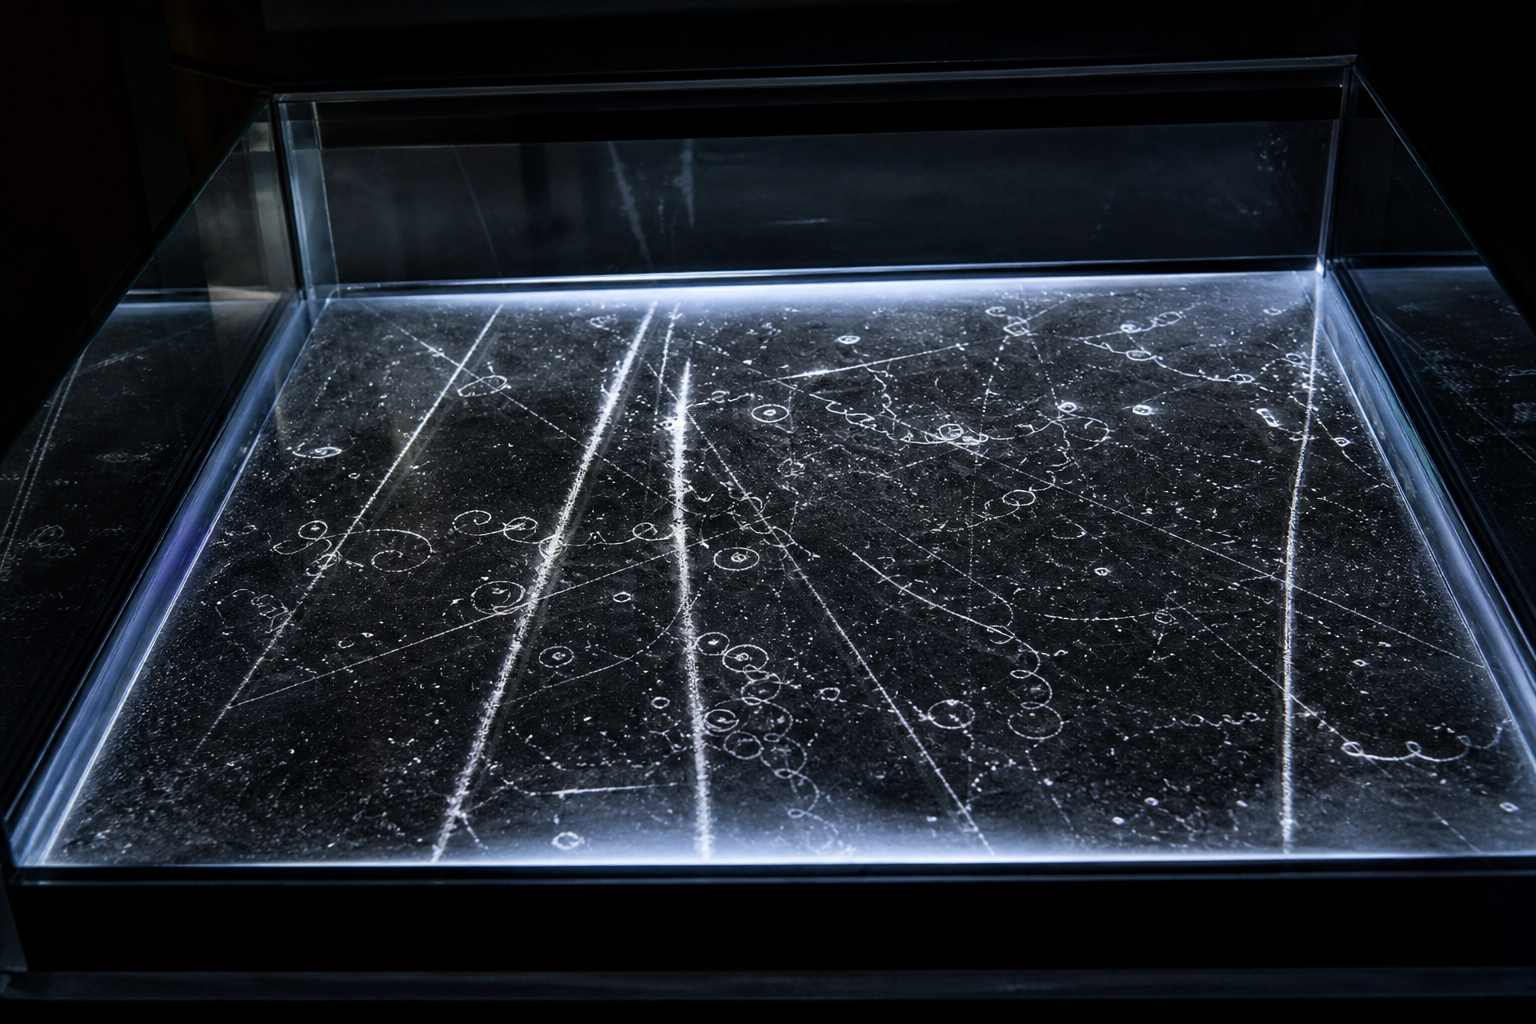
\includegraphics[width=0.58\linewidth]{images/book5/ai/b5-05-cloud-chamber.png}

{\small Geladen deeltjes die een nevelvat doorkruisen. Sporen als deze --- krullend in magneetvelden, in paren verschijnend --- maakten van $E = mc^2$ een formule die dagelijkse boekhouding werd: het positron is op zo'n foto ontdekt.}
\end{omfigure}

\section{Opgaven}

\begin{exercise}[$\star$]\label{exo:b3:relativistic-dynamics:1}
Een elektron ($mc^2 = \qty{0.511}{MeV}$) beweegt met $0.99c$. Bereken
$\gamma$, zijn impuls in $\unit{MeV}/c$, en zijn totale en kinetische
energie. Dezelfde vragen voor een proton ($mc^2 = \qty{938}{MeV}$) met
kinetische energie \qty{1}{GeV}.
\end{exercise}

\begin{exercise}[$\star$]\label{exo:b3:relativistic-dynamics:2}
(a) Hoeveel energie sluimert er in één gram materie? (b) De explosie van
Hiroshima maakte ongeveer \qty{6e13}{J} vrij: welk massaverschil is dat?
(c) De zon straalt $L = \qty{3.8e26}{W}$ uit: hoeveel massa verliest zij
per seconde, en welk deel van haar $\qty{2e30}{kg}$ in tien miljard jaar?
(d) De accu van uw telefoon slaat \qty{5e4}{J} op: hoeveel zwaarder is
een opgeladen telefoon?
\end{exercise}

\begin{exercise}[$\star$]\label{exo:b3:relativistic-dynamics:3}
(a) Hoeveel impuls draagt de bundel van een laserpen van \qty{5}{mW} per
seconde, en welke kracht voelt de pen? (b) Welke kracht oefent zonlicht
(\qty{1.4}{kW/m^2}) uit op een perfect spiegelend zonnezeil van
\qty{100}{m^2}? (c) Hoe snel beweegt een zeilschip van \qty{10}{kg} na
een maand vanuit rust? (d) Waarom wijst de stofstaart van een komeet van
de zon af?
\end{exercise}

\begin{exercise}[$\star$]\label{exo:b3:relativistic-dynamics:4}
Oefening met eenheden. (a) Toon aan dat $\unit{MeV}/c^2$ een
massa-eenheid is en zet de elektronmassa om naar kilogram. (b) Hoeveel is
\qty{1}{GeV/c} in $\unit{kg.m/s}$? (c) Een kwadraat van een \omterm{def:b3:relativistic-dynamics:four-momentum}{invariante
massa} komt uit op $s = \qty{16}{GeV^2}$ (in eenheden met $c = 1$): welke
energie in het impulsmiddelpuntstelsel is dat? (d) Waarom stellen
deeltjesfysici $c = 1$, en wat moet een lezer terugzetten om
SI-getallen te krijgen?
\end{exercise}

\begin{exercise}[$\star\star$]\label{exo:b3:relativistic-dynamics:5}
De elektronen van Bertozzi hadden kinetische energieën $0.5$, $1$, $4.5$
en \qty{15}{MeV}. (a) Bereken voor elk de voorspelling van Newton $v^2 = 2E_k/m$, in eenheden $c^2$. (b) Bereken de relativistische $v^2/c^2$. (c)
Zijn vluchttijd over \qty{8.4}{m} bij \qty{15}{MeV}: wat wees de klok
aan, en wat zou Newton hebben voorspeld? (d) De energie van de elektronen
werd ook calorimetrisch gemeten --- aan hun warmte bij de inslag: waarom
was die stap het eigenlijke punt van het experiment?
\end{exercise}

\begin{exercise}[$\star\star$]\label{exo:b3:relativistic-dynamics:6}
Het geladen pion vervalt in rust: $\pi^+ \to \mu^+\nu$, $m_\pi c^2 =
\qty{139.6}{MeV}$, $m_\mu c^2 = \qty{105.7}{MeV}$, $m_\nu \approx 0$.
(a) Toon aan dat $pc = (m_\pi^2 - m_\mu^2)c^4/2m_\pi c^2$ en reken het
uit. (b) De kinetische energie en de snelheid van het muon. (c) De
energie van het neutrino. (d) Wat zijn in vlucht bij $\gamma_\pi = 50$ de
maximale en de minimale labenergie van het vervalmuon (verval voorwaarts
en achterwaarts)?
\end{exercise}

\begin{exercise}[$\star\star$]\label{exo:b3:relativistic-dynamics:7}
\omterm{def:b3:relativistic-dynamics:four-momentum}{Invariante massa} in \omterm{def:b3:lagrangian-mechanics:action}{actie}. (a) Twee fotonen van elk \qty{200}{MeV}
vliegen onder $60^\circ$ ten opzichte van elkaar: bereken de \omterm{def:b3:relativistic-dynamics:four-momentum}{invariante
massa} van het paar. (b) Een neutraal pion ($m_{\pi^0}c^2 = \qty{135}{MeV}$) vervalt in twee fotonen: wat is de \omterm{def:b3:relativistic-dynamics:four-momentum}{invariante massa} van
het fotonpaar, in elk stelsel? (c) Leg uit hoe een experiment een deeltje
``ontdekt'' als een bult in de verdeling van de \omterm{def:b3:relativistic-dynamics:four-momentum}{invariante massa} van zijn
vervalproducten. (d) Twee fotonen met gelijke energie vliegen precies
evenwijdig: \omterm{def:b3:relativistic-dynamics:four-momentum}{invariante massa}? Wat zegt dit over het ruststelsel van een
lichtbundel?
\end{exercise}

\begin{exercise}[$\star\star$]\label{exo:b3:relativistic-dynamics:8}
Boekhouding van de LHC (protonen met $E = \qty{6.8}{TeV}$). (a) $\gamma$,
en het snelheidstekort $c - v$ (gebruik $c - v \approx c/2\gamma^2$). (b)
De omloopfrequentie op de ring van \qty{27}{km} en het aantal rondjes per
seconde. (c) De opgeslagen energie van een bundel van \num{3e14} protonen,
in kilogram TNT (\qty{4.2e6}{J/kg}). (d) Het massa-equivalent van de
kinetische energie van de twee bundels, in microgram --- materie die op
het punt staat gemaakt te worden.
\end{exercise}

\begin{exercise}[$\star\star$]\label{exo:b3:relativistic-dynamics:9}
Botsende fotonen. (a) Toon aan dat één foton in vacuüm niet in een paar
elektron--positron kan vervallen, hoe energierijk ook (gebruik de
invariant). (b) Toon aan dat paarvorming tegen een tweede foton met
energie $\epsilon$ frontaal $E\epsilon \ge (m_{\text{e}}c^2)^2$ vergt.
(c) Welke partner heeft een foton van \qty{511}{keV} nodig? En een
röntgenfoton van \qty{50}{keV}? (d) Het heelal is gevuld met sterrenlicht
en met de kosmische achtergrondstraling: wat voorspelt (b) voor het
bereik van $\gamma$-straling van TeV door de intergalactische ruimte?
\end{exercise}

\begin{exercise}[$\star\star\star$]\label{exo:b3:relativistic-dynamics:10}
Compton, met viererimpulsen. Een foton met golflengte $\lambda$ treft een
elektron in rust en verstrooit onder de hoek $\theta$. (a) Schrijf het
behoud van \omterm{def:b3:relativistic-dynamics:four-momentum}{viererimpuls} op en isoleer de invariant van het uiteindelijke
elektron. (b) Leid af dat
\[
\lambda' - \lambda = \frac{h}{m_{\text{e}}c}\,(1 - \cos\theta) .
\]
(c) Bereken $h/m_{\text{e}}c$ en de maximale verschuiving; waarom is het
effect met zichtbaar licht onzichtbaar maar bij röntgenstraling
doorslaggevend? (d) Wat stelde Comptons meting van 1923 over het licht
vast dat het foto-elektrisch effect niet had vastgesteld?
\end{exercise}

\begin{exercise}[$\star\star\star$]\label{exo:b3:relativistic-dynamics:11}
Het einde van het spectrum van de kosmische straling. Het heelal baadt in
microgolffotonen met een typische energie $\epsilon = \qty{6e-4}{eV}$.
Een proton met energie $E$ dat er frontaal een treft kan tot de
$\Delta$-resonantie worden aangeslagen ($m_\Delta c^2 = \qty{1232}{MeV}$) en verliest daarbij telkens energie. (a) Toon aan dat
de drempelvoorwaarde bij benadering $4E\epsilon =
(m_\Delta^2 - m_{\text{p}}^2)c^4$ luidt. (b) Bereken de drempel $E$. (c) Daarboven is
het heelal ondoorzichtig voor protonen voorbij zo'n \qty{100}{Mly}: wat
voorspelt dit voor het waargenomen spectrum van de kosmische straling (de
afsnijding van Greisen, Zatsepin en Kuzmin)? (d) Er is kosmische straling
van $\qty{3e20}{eV}$ geregistreerd --- ``Oh-My-God''-deeltjes: wat eist
hun bestaan van hun bronnen?
\end{exercise}

\begin{exercise}[$\star\star\star$]\label{exo:b3:relativistic-dynamics:12}
De fotonraket. Een raket met beginmassa $m_{\text{i}}$ stoot haar
uitlaatstroom als een gebundelde lichtstraal uit en haalt de snelheid
$\beta c$. (a) Toon met behoud van energie en impuls tussen begin en eind
aan dat
\[
\frac{m_{\text{i}}}{m_{\text{f}}} =
\sqrt{\frac{1 + \beta}{1 - \beta}} = \eu^{\varphi} ,
\]
de exponentiële functie van de snelheidshoek --- de relativistische
vergelijking van Tsiolkovski met de best mogelijke uitlaat. (b)
Massaverhouding om $0.9c$ te halen? En om $0.9c$ te halen én op de
bestemming te \emph{stoppen}? (c) De bundel moet ergens vandaan komen:
hoeveel kilogram antimaterie per kilogram nuttige lading kost de enkele
reis naar $0.9c$ bij annihilatie van materie en antimaterie met perfect
rendement? (d) De wereldproductie van antiprotonen bedraagt nanogrammen
per jaar: concludeer in één zin over fotonraketten.
\end{exercise}

\begin{omfigure}
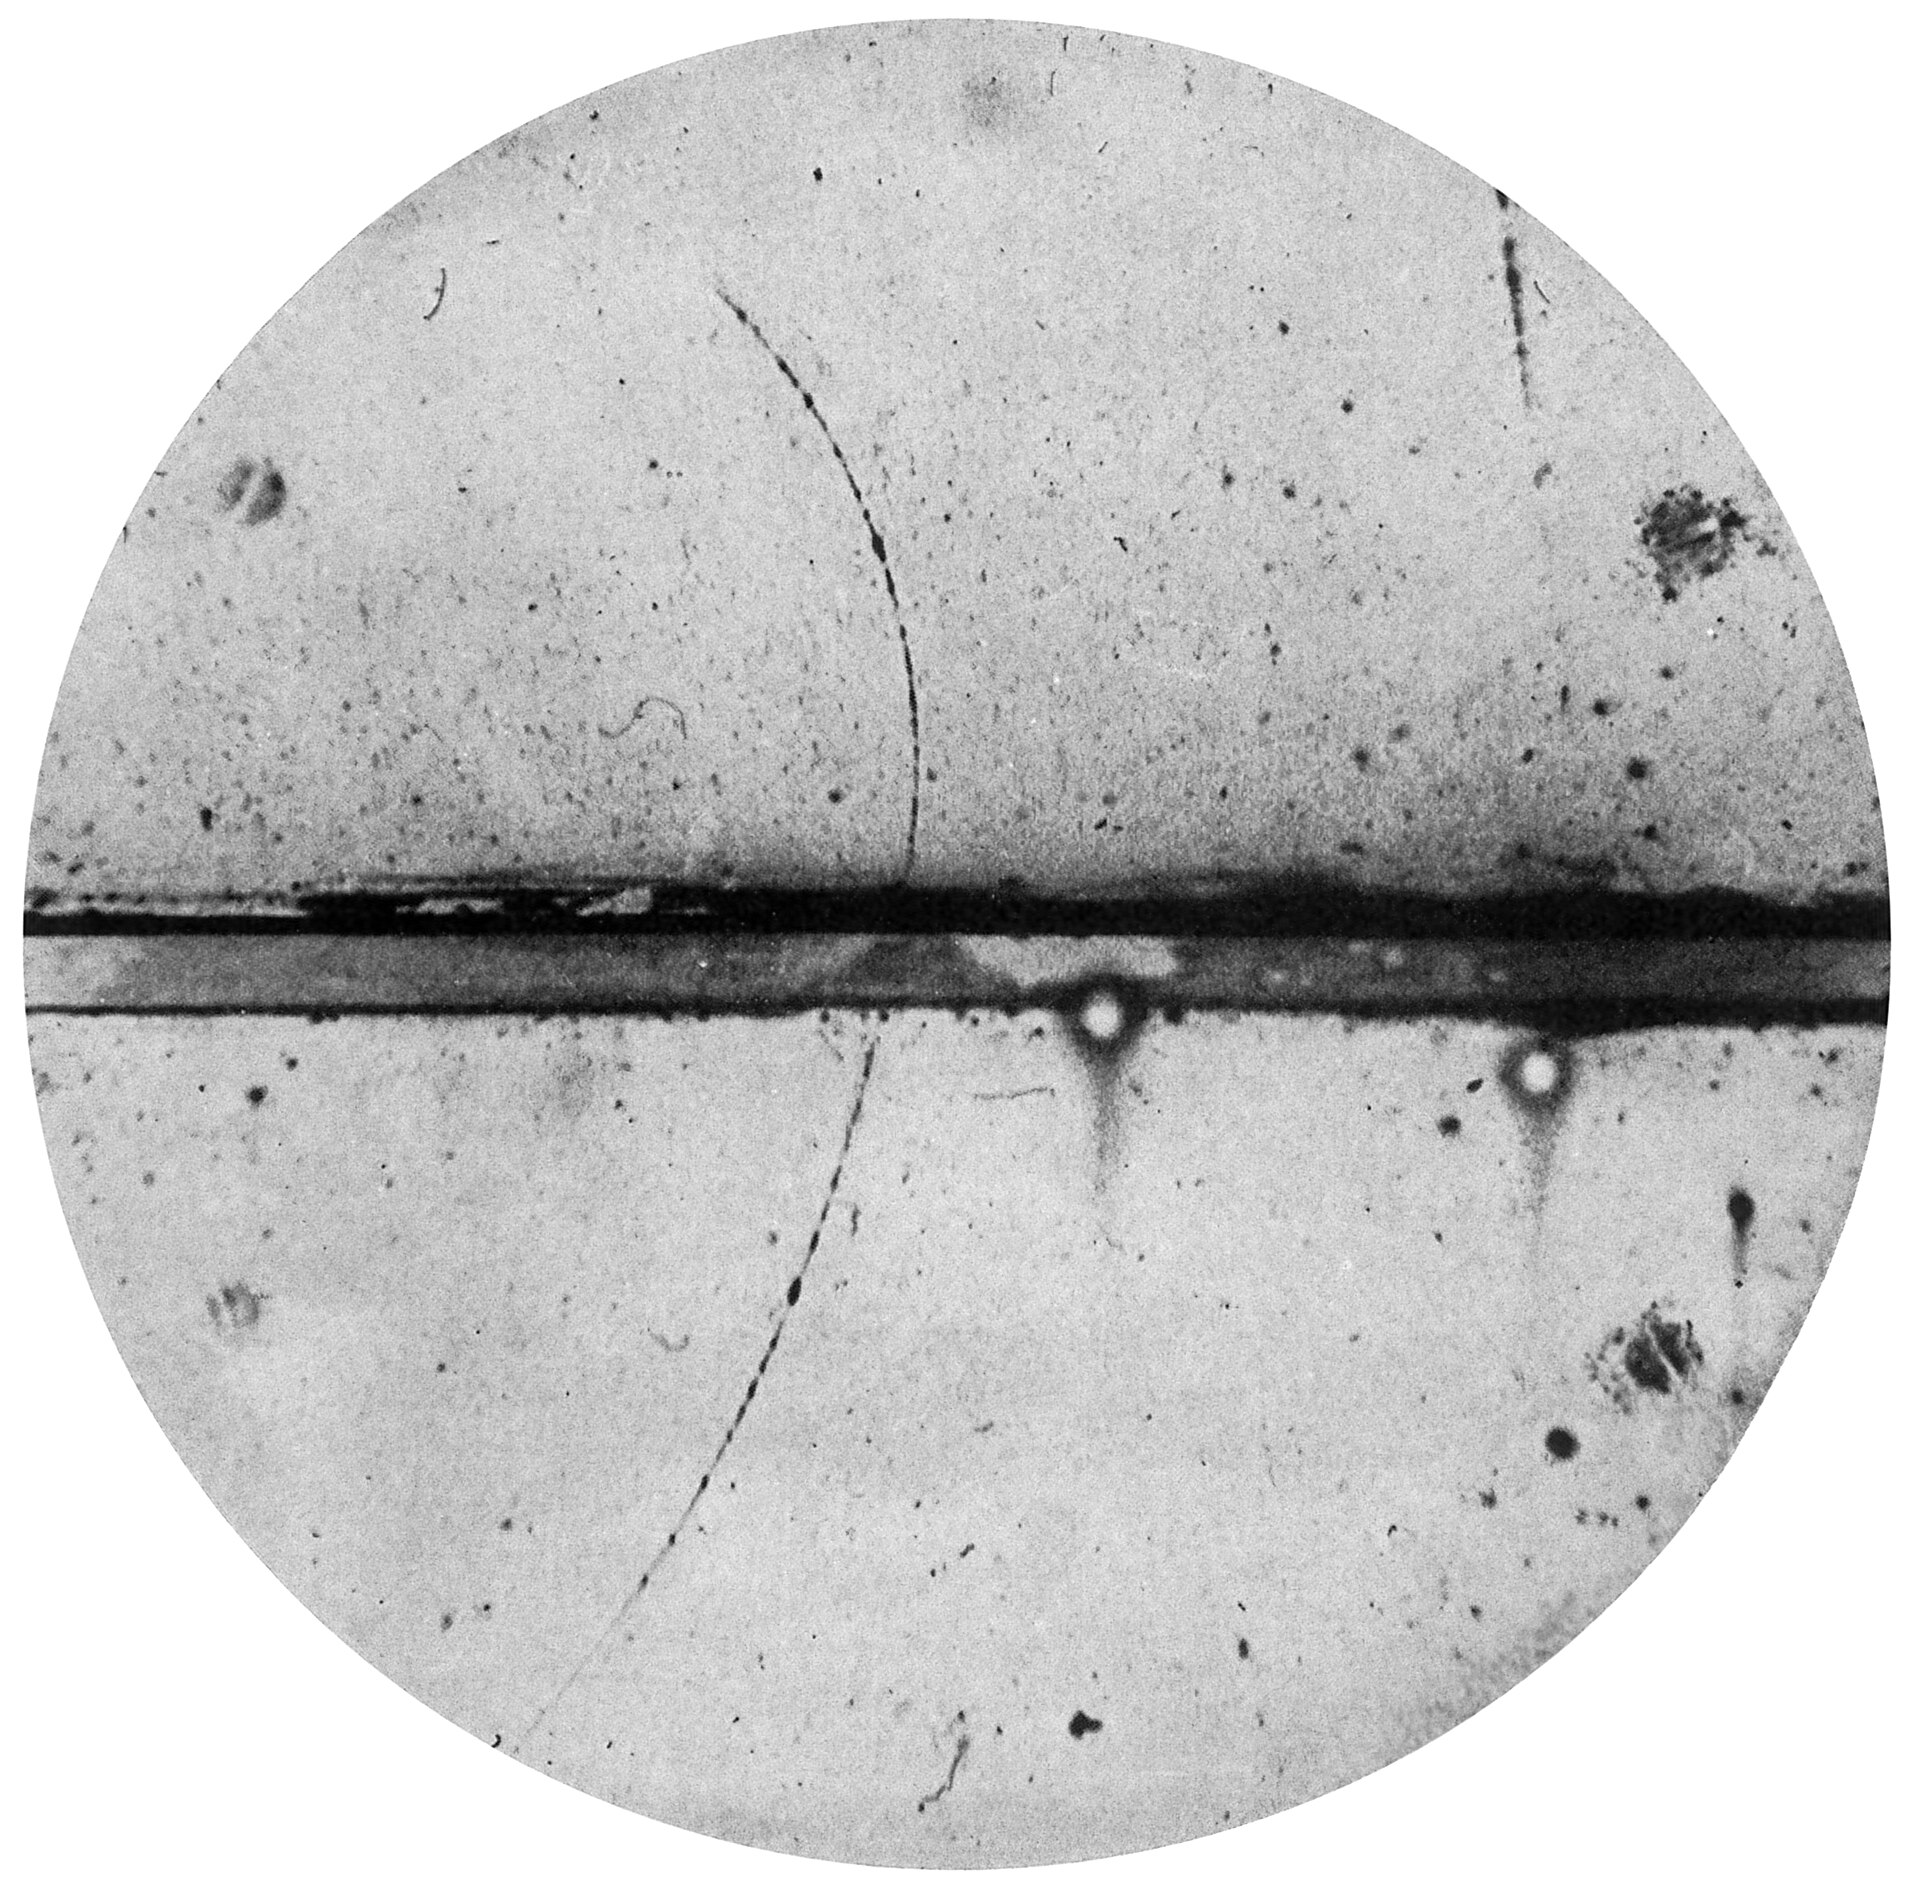
\includegraphics[width=0.5\linewidth]{images/book5/photo-positron-anderson.jpg}

{\small De ontdekking van de antimaterie (Carl D. Anderson, 1932, publiek domein): één positron dat door de loden plaat van het nevelvat omhoog klimt, de verkeerde kant op krommend voor een elektron en te strak voor een proton --- de boekhouding van $E = mc^2$ betrapt op achteruitlopen.}
\end{omfigure}

\section{Vraagstuk: Materie maken --- het antiproton en het Bevatron}

\begin{problem}[{Weekendvraagstuk --- hoe het impulsbehoud de
antiwereld beprijsde}]\label{pb:b3:relativistic-dynamics:1}
De vergelijkingen van Dirac eisten vanaf 1931 dat het proton een
spiegeltweeling met tegengestelde lading had. Er een maken betekende zijn
\omterm{def:b3:relativistic-dynamics:momentum-energy}{rustenergie} met bundelenergie kopen --- en het impulsbehoud stelde de
prijs. Dit vraagstuk beprijst haar, ontwerpt de machine die haar betaalde
en volgt de ontdekking van 1955. Gegevens: $m_{\text{p}}c^2 = \qty{938.3}{MeV}$; lading en \emph{baryongetal} (protonen en neutronen
$+1$, antiprotonen $-1$) blijven in elke reactie behouden.

\medskip\noindent\textbf{Deel I --- Het gereedschap van de \omterm{def:b3:relativistic-dynamics:four-momentum}{viererimpuls}.}
\begin{enumerate}
  \item Toon voor één deeltje aan dat $E^2 - p^2c^2 = m^2c^4$ uit de
        definities van $E$ en $\vect p$ volgt.
  \item Waarom is $E_{\text{tot}}^2 -
        p_{\text{tot}}^2c^2$ voor een
        stelsel in alle stelsels hetzelfde, en waaraan is het gelijk in
        het impulsmiddelpuntstelsel?
  \item Een protonbundel met energie $E$ treft een proton in rust: toon
        aan dat $M^2c^4 = 2m_{\text{p}}^2c^4 + 2E\,m_{\text{p}}c^2$.
  \item Toets de twee limieten: bij lage energie $Mc^2 \to
        2m_{\text{p}}c^2$; bij hoge energie $Mc^2 \approx
        \sqrt{2E\,m_{\text{p}}c^2}$ --- de wortelwet.
  \item Een reactie is alleen toegestaan als $Mc^2$ de opgetelde
        rustmassa's van de producten haalt, waarbij bij de drempel alle
        producten in het impulsmiddelpuntstelsel in rust zijn:
        rechtvaardig die laatste toevoeging.
  \item Waarom kan de kinetische energie van de producten in het lab bij
        een vast trefplaatje nooit voor deeltjesvorming worden
        teruggewonnen?
\end{enumerate}

\medskip\noindent\textbf{Deel II --- Het antiproton beprijzen.}
\begin{enumerate}[resume]
  \item Bij botsingen $p + p$ moet de goedkoopste reactie die een
        antiproton $\bar p$ maakt ook een \emph{extra} proton maken:
        schrijf haar op en rechtvaardig dit met lading en baryongetal.
  \item Toon aan dat de drempel $Mc^2 = 4m_{\text{p}}c^2$ vergt.
  \item Leid de vereiste bundelenergie $E = 7m_{\text{p}}c^2$ en de
        kinetische energie $T = 6m_{\text{p}}c^2$ af; bereken $T$.
  \item Welk deel van de kinetische energie van de bundel werd bij de
        drempel werkelijk nieuwe rustmassa ($2m_{\text{p}}c^2$ ervan)?
        Waar zit de rest?
  \item Welke kinetische energie \emph{per bundel} zou dezelfde reactie
        in een frontale botser $p$--$p$ nodig hebben? Vergelijk de twee
        ontwerpen.
  \item In 1954 bestond er geen botser (de bundels waren te ijl om
        elkaar te raken): welk praktisch feit dwong tot de keuze voor
        een vast trefplaatje, en wat kostte dat aan bundelenergie?
\end{enumerate}

\medskip\noindent\textbf{Deel III --- Het Bevatron ontwerpen.}
De machine die in Berkeley werd gebouwd haalde $T = \qty{6.2}{GeV}$ ---
ruim boven de drempel --- met dipoolvelden van $B =
\qty{1.56}{T}$.
\begin{enumerate}[resume]
  \item Bereken de totale energie en de impuls van de bundel bij
        topenergie.
  \item Bereken de buigstraal $r = p/qB$ en vergelijk met de
        \qty{15.2}{m} van de machine.
  \item Bereken de snelheid van het proton en de omloopfrequentie op de
        ring met omtrek $2\pi r$.
  \item Bij injectie komen de protonen aan met \qty{10}{MeV} kinetische
        energie: bereken hun snelheid en leg uit waarom de
        versnelfrequentie tijdens elke cyclus moest \emph{meelopen}
        (welke twee grootheden veranderen als $E$ groeit?).
  \item Met ongeveer \qty{1.5}{kV} winst per omloop: hoeveel omlopen
        duurt één versnelcyclus, en hoe lang?
  \item De naam ``Bevatron'' kwam van BeV, miljarden elektronvolt:
        formuleer in één regel welke natuurkunde het ontwerpgetal van
        $6$ en een fractie BeV vastlegde.
\end{enumerate}

\medskip\noindent\textbf{Deel IV --- De ontdekking, 1955.}
\begin{enumerate}[resume]
  \item Een magneet buigt elke kandidaat op een cirkel: leg uit waarom
        dit deeltjes op \emph{impuls} selecteert ($r = p/qB$) en niet op
        energie of snelheid --- en waarom een op impuls geselecteerde
        bundel toch soorten mengt.
  \item De bundel op een koperen trefplaatje maakte stromen negatieve
        pionen ($m_\pi c^2 = \qty{139.6}{MeV}$) waartussen enkele
        antiprotonen schuilgingen. De spectrometer selecteerde negatieve
        deeltjes met impuls $p = \qty{1.19}{GeV}/c$: bereken bij die
        impuls de snelheid van een antiproton en die van een pion.
  \item Bereken de twee vluchttijden over het traject van \qty{12}{m}:
        welke tijdsresolutie had de ontdekking nodig?
  \item Een tweede, onafhankelijke handtekening gebruikte
        \v cerenkovtellers, die pas boven een snelheidsdrempel
        aanslaan: welk deeltje werd geacht ze te laten aanslaan, en
        waarom telt redundantie bij een ontdekking?
  \item Chamberlain en Segrè telden ongeveer één antiproton per
        $\num{44000}$ pionen: waarom garandeerde het drempelargument dat
        het tempo ook boven de drempel minuscuul zou zijn?
  \item Een antiproton ontmoet uiteindelijk een proton en annihileert:
        hoeveel energie komt er per gebeurtenis vrij, en typisch waarin?
  \item Vat het genoemde resultaat samen: het behoud van \omterm{def:b3:relativistic-dynamics:four-momentum}{viererimpuls}
        beprijsde het antiproton op $T = 6m_{\text{p}}c^2 =
        \qty{5.6}{GeV}$ op een vast trefplaatje; een synchrotron van
        \qty{6.2}{GeV} en \qty{15}{m} betaalde die prijs, en de
        antiwereld werd laboratoriumfeit --- de Nobelprijs van 1959.
\end{enumerate}
\end{problem}
